\documentclass[12pt]{exam}
%\documentclass[12pt]{article}
\usepackage[letterpaper, margin=0.75in]{geometry}
\usepackage{graphicx}
\usepackage{enumitem}
\usepackage{booktabs}
\usepackage{amsmath}
\usepackage{tabularx}

\begin{document}
\footer{}{Page \thepage\ of \numpages}{}

\begin{flushright}
\makebox[0.5\textwidth]{\large Name:\enspace\hrulefill}
\vspace{0.2in}

\makebox[0.5\textwidth]{\large Date:\enspace\hrulefill}
\end{flushright}

\begin{center}
\includegraphics[width=10cm]{../images/logo.png}
\end{center}

\begin{center}
\noindent{\LARGE Conceptual Physics \\ Class 4 Questions \\ Feb. 23, 2018 \\}
\end{center}
\vspace{0.2in}

\clearpage

\begin{questions}
\question
Plot the following $(t, x)$ ordered pairs on the graph below. Make sure you label your axes.

$(1, 5)$ $(-2, -4)$ $(-3, 1)$ $(6, -2)$ $(3, 2.5)$

\begin{center}
\includegraphics[width=\linewidth]{../images/coop3_grid.png}
\end{center}

\clearpage
\question
Consider the following \textbf{position} versus time graph for some object. 

\begin{center}
\includegraphics{../images/coop2_posVsTime.pdf}
\end{center}

\begin{parts}
	\part At which point(s) is the object not moving?
	\vspace{0.1in}
	\part At which point(s) is the object moving at a constant velocity?
	\vspace{0.1in}
	\part At which point(s) is the object moving with a positive velocity?
	\vspace{0.1in}
	\part At which point(s) is the object moving with a negative velocity?
	\vspace{0.1in}
	\part At which point(s) does the object experience zero acceleration?
\end{parts}
\vspace{0.2in}
\question
Now, let consider the following \textbf{velocity} versus time graph for some object.

\begin{center}
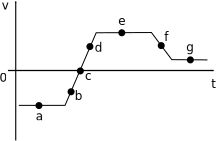
\includegraphics{../images/coop2_velVsTime.pdf}
\end{center}

\begin{parts}
	\part At which point(s) is the object not moving?
	\vspace{0.1in}
	\part At which point(s) is the object moving at a constant velocity?
	\vspace{0.1in}
	\part At which point(s) is the object moving with a positive velocity?
	\vspace{0.1in}
	\part At which point(s) is the object moving with a negative velocity?
	\vspace{0.1in}
	\part At which point(s) does the object experience zero acceleration?
	\vspace{0.1in}
	\part At which point(s) does the object experience positive acceleration?
	\vspace{0.1in}
	\part At which point(s) does the object negative acceleration?
\end{parts}
\clearpage

\question
What is wrong with this plot?

\begin{center}
\includegraphics[width=0.8\linewidth]{../images/coop3_labels.png}
\end{center}

\question Consider the following two graphs of position versus time for some object. What is strange about each of them? (From \textit{Light and Matter}, Chapter 2, discussion question E)
	
\begin{table}[h!]
     \begin{center}
     \begin{tabularx}{\textwidth}{ X X }
     
     (a) \raisebox{-\totalheight}{\includegraphics[width=0.45\textwidth]{../images/hw2WeirdPosition1.pdf}}
      & 
      (b) \raisebox{-\totalheight}{\includegraphics[width=0.45\textwidth]{../images/hw2WeirdPosition2.pdf}}\\
      \end{tabularx}
      \end{center}
\end{table}

\clearpage
\question The Shinkansen is a network of high-speed railway lines in Japan. The trains reach a maximum operating speed of 320~km/h (200~mph), although in April 2015 one set the world record 603 km/h (375 mph).

One of these high-speed trains accelerates (assume constant acceleration) from rest at a station, reaching its maximum operating speed ($3.20\times 10^2$~ km/h) in 1.00~minutes. It continues to cruise at this speed for 10.0 minutes, then slows down to a stop during the course of one more minute to reach the next station (assume constant deceleration). After waiting 5 minutes for passengers to embark/disembark, it returns to its original stop by performing the same course in reverse: accelerating to $3.20\times 10^2$~km/h in 1.00~minutes, cruising for 10.0 minutes and slowing down to a stop in another minute.
\vspace{0.5in}
\begin{parts}
	\part Using the grid below, plot the train's \textbf{velocity} as a function of \textbf{time}.
\begin{center}
\includegraphics[width = 0.9\textwidth]{../images/grid.png}
\end{center}
\clearpage
	\part Using the grid below, plot the train's \textbf{acceleration} as a function of \textbf{time}.
\begin{center}
\includegraphics[width = 0.9\textwidth]{../images/grid.png}
\end{center}
	\clearpage
	\part Using the grid below, plot the train's \textbf{position} as a function of \textbf{time}.
\begin{center}
\includegraphics[width = 0.9\textwidth]{../images/grid.png}
\end{center}




\end{parts}

\end{questions}

\end{document}

